\pdfoutput=1
% \documentclass[red,handout,professionalfont]{beamer}
\documentclass[red,professionalfont]{beamer}
\usepackage{multimedia}
\usepackage{chessboard}
\usepackage{url}
\usepackage{amssymb}  % the check symbol 
% Python listing setup

\usepackage{color}
\usepackage[procnames]{listings}
\usepackage{textcomp}
\usepackage{setspace}
\usepackage{palatino}
\renewcommand{\lstlistlistingname}{Code Listings}
\renewcommand{\lstlistingname}{Code Listing}
\definecolor{gray}{gray}{0.5}
\definecolor{green}{rgb}{0,0.5,0}
\definecolor{lightgreen}{rgb}{0,0.7,0}
\definecolor{purple}{rgb}{0.5,0,0.5}
\definecolor{darkred}{rgb}{0.5,0,0}
\lstnewenvironment{python}[1][]{
\lstset{
language=python,
breaklines=true,
basicstyle=\ttfamily\small\setstretch{1},
stringstyle=\color{green},
showstringspaces=false,
alsoletter={1234567890},
otherkeywords={\ , \}, \{},
keywordstyle=\color{blue},
emph={access,and,as,break,class,continue,def,del,elif,else,%
except,exec,finally,for,from,global,if,import,in,is,%
lambda,not,or,pass,print,raise,return,try,while,assert},
emphstyle=\color{orange}\bfseries,
emph={[2]self},
emphstyle=[2]\color{gray},
emph={[4]ArithmeticError,AssertionError,AttributeError,BaseException,%
DeprecationWarning,EOFError,Ellipsis,EnvironmentError,Exception,%
False,FloatingPointError,FutureWarning,GeneratorExit,IOError,%
ImportError,ImportWarning,IndentationError,IndexError,KeyError,%
KeyboardInterrupt,LookupError,MemoryError,NameError,None,%
NotImplemented,NotImplementedError,OSError,OverflowError,%
PendingDeprecationWarning,ReferenceError,RuntimeError,RuntimeWarning,%
StandardError,StopIteration,SyntaxError,SyntaxWarning,SystemError,%
SystemExit,TabError,True,TypeError,UnboundLocalError,UnicodeDecodeError,%
UnicodeEncodeError,UnicodeError,UnicodeTranslateError,UnicodeWarning,%
UserWarning,ValueError,Warning,ZeroDivisionError,abs,all,any,apply,%
basestring,bool,buffer,callable,chr,classmethod,cmp,coerce,compile,%
complex,copyright,credits,delattr,dict,dir,divmod,enumerate,eval,%
execfile,exit,file,filter,float,frozenset,getattr,globals,hasattr,%
hash,help,hex,id,input,int,intern,isinstance,issubclass,iter,len,%
license,list,locals,long,map,max,min,object,oct,open,ord,pow,property,%
quit,range,raw_input,reduce,reload,repr,reversed,round,set,setattr,%
slice,sorted,staticmethod,str,sum,super,tuple,type,unichr,unicode,%
vars,xrange,zip},
emphstyle=[4]\color{purple}\bfseries,
upquote=true,
morecomment=[s][\color{lightgreen}]{"""}{"""},
commentstyle=\color{red}\slshape,
literate={>>>}{\textbf{\textcolor{darkred}{>{>}>}}}3%
         {...}{{\textcolor{gray}{...}}}3,
procnamekeys={def,class},
procnamestyle=\color{blue}\textbf,
framexleftmargin=1mm, framextopmargin=1mm,% frame=shadowbox,
%rulesepcolor=\color{blue},
#1
}}{}


\usepackage{tikz}
\usepackage{tikz-qtree}
\usetikzlibrary{decorations.pathreplacing,positioning}
%\bibliography{mujstyl}
\theoremstyle{definition}
\newtheorem{definice}{Definition}[section]
\newtheorem{thm}{Theorem}[section]
\newtheorem{idea}{Idea}[section]
\newtheorem{cor}[thm]{Corrollary}
\newtheorem{lem}[thm]{Lemma}
\newtheorem{obs}[thm]{Observation}
\newtheorem{rem}[thm]{Remark}
\newtheorem{ex}[thm]{Example}
\newtheorem{quizz}[thm]{Question}
\newcommand{\pomega}{\mbox{$\mathcal{P}(\omega)$}}
\newcommand{\cont}{\mbox{$\mathfrak c$}}
\newcommand{\ba}{\mbox{${\mathbb B}$}}
\newcommand{\0}{\mbox{${\bf 0}$}}
\newcommand{\F}{\mbox{${\mathcal F}$}}
\newcommand{\rest}{\mbox{$\upharpoonright$}}
\newcommand{\cl}[1]{\mbox{$\overline{#1}$}}
\newcommand{\yes}{\textcolor{green}{$\checkmark$}}
\newcommand{\no}{\textcolor{red}{$\times$}}
\renewcommand{\emph}[1]{{\bf #1}}
\mode<presentation>
{
\useinnertheme{rounded}

\usecolortheme{whale}
\usecolortheme{orchid}

\setbeamerfont{block title}{size={}}

%   \useoutertheme{default}
%   \usetheme{Copenhagen}
%   \useoutertheme{default}
  \setbeamercovered{invisible}
}
\setbeamertemplate{navigation symbols}{} 
\usepackage[utf8]{inputenc}
\usepackage[czech,english]{babel}
\usepackage{lmodern}
%\usepackage{times}
\usepackage[T1]{fontenc}


\tikzset{onslide/.code args={<#1>#2}{%
  \only<#1>{\pgfkeysalso{#2}} % \pgfkeysalso doesn't change the path
}}

\tikzstyle{hilight}=[red,ultra thick]
\tikzstyle{active}=[yellow,ultra thick]
\tikzstyle{memory}=[blue]



\title[]{Neuronové sítě\\ (11. přednáška)}

% Dnes se podíváme na jednoduché "goal-based" agenty
% a ukážeme si obecné postupy 


% \author[]{Jonathan L. Verner}
% \institute[Charles University, Prague] % (optional,but mostly needed)
% {
%   Department of Logic\\
  %   Faculty of Philosophy\\
%   Charles University in Prague
% }
\date[]{}
% \subject{}
%\pgfdeclareimage[height=1cm]{university-logo}{UK-logo}
%\logo{\pgfuseimage{university-logo}}

\begin{document}

\AtBeginSection[]
{
  \begin{frame}<beamer>
    \begin{block}{}
%    \begin{centering}
    \hfill\insertsection\hfill\
 %   \end{centering}
    \end{block}
    %\tableofcontents[currentsection]
  \end{frame}
}

\AtBeginSubsection[]
{
  \begin{frame}<beamer>
    \begin{block}{}
  %  \begin{centering}
    \hfill\insertsubsection\hfill\
   % \begin{centering}
    \end{block}
    %\tableofcontents[currentsection]
  \end{frame}
}

%#################################################################

\begin{frame}{} \titlepage
%{\ \hfill \includegraphics[width=1cm]{UK-logo}\hfill\ }
\end{frame}

\begin{frame}\frametitle{Machine Learning --- Naučit stroje se učit}
\alert{O co jde?}\pause

Máme \emph{model výpočtu}\pause\ (t.j. výpočetní postup jednoznačně daný
vstupy a nějakými parametry)\pause, chceme najít vhodné nastavení parametrů,
aby postup (model) dával řešení našeho problému.\pause

\vskip0.3cm
\alert{Příklad}

 Chceme převést stupně Celsia na stupně Farenheita.\pause\
 Modelem výpočtu bude lineární funkce $f(x) = \alpha x + b$\pause, která je daná dvěma
 parametry --- $\alpha, b$. \pause\ Vhodné nastavení parametrů v tomto případě je $\alpha=9/5$ a $b=32$.\pause\

\vskip0.3cm
Při strojovém učení zvolíme dostatečně silný model\pause\ a nastavení parametrů chceme nalézt automaticky na základě vzorových řešení
daného problému\pause\ (např. víme, že $0^oC = 32^oF$ a $100^o C = 212^o F$).\pause

\end{frame}

\begin{frame}\frametitle{Strojové učení --- Proč}
\begin{center}
 Slogan
\end{center}\pause
\begin{block}{}
 \begin{center} 
  Chceme, aby se stroj naučil řešit zadaný problém na základě vzorových řešení
 \end{center}
\end{block}\pause
\begin{itemize}
 \item řešení je příliš komplikované\pause
 \item problém se často mění, vyvíjí\pause
 \item lidská práce je drahá (v porovnání se strojovou)
\end{itemize}
\end{frame}
% The Machine Learning Approach 
% • Instead of writing a program by hand for each specific task, we collect 
% lots of examples that specify the correct output for a given input. 
% • A machine learning algorithm then takes these examples and produces 
% a program that does the job. 
% – The program produced by the learning algorithm may look very 
% different from a typical hand-written program. It may contain millions 
% of numbers. 
% – If we do it right, the program works for new cases as well as the ones 
% we trained it on. 
% – If the data changes the program can change too by training on the 
% new data. 
% • Massive amounts of computation are now cheaper than paying 
% someone to write a task-specific program.

\begin{frame}\frametitle{Strojové učení --- typické aplikace}
\begin{itemize}
 \item Rozpoznávání vzorců\pause
 \begin{itemize}
 \item věci na fotkách\pause
 \item osoby na fotkách\pause
 \item výrazy tváře\pause
 \item mluvená slova\pause
 \end{itemize}
 \item Rozpoznávání anomálií\pause
 \begin{itemize}
 \item netypické sekvence finančních transakcí\pause
 \item netypická data přicházející ze senzorů v atomové elektrárně\pause
 \end{itemize}
 \item Předpovídání
 \begin{itemize}
 \item vývoj ceny akcií na burze / vývoj měnového kurzu\pause
 \item jaké filmy bude mít daný člověk rád
 \end{itemize}
\end{itemize}
\end{frame}

\begin{frame}\frametitle{Strojové učení --- příklad}
\begin{center}
 Rozpoznávání věcí na fotkách\\
 {\tiny(zdroj: G. Hinton, Neural Networks for ML)}
\end{center}\pause
\begin{center}
\begin{minipage}{3cm}
\includegraphics[width=2.5cm]{ML/krepelka.png}
\begin{itemize}
\item[40] vydra
\item[15] \alt<3->{\alert{křepelka}}{křepelka}
\item[7] tetřev
\item[6] koroptev
\end{itemize}\pause
\end{minipage}\pause
\begin{minipage}{3.5cm}
\includegraphics[width=2.5cm]{ML/pluh.png}
\begin{itemize}
\item[85] \alt<5->{\alert{sněžný pluh}}{sněžný pluh}
\item[6] vrtná plošina
\item[6] záchranný člun
\item[2] popelářské auto
\end{itemize}\pause
\end{minipage}\pause
\begin{minipage}{3.5cm}
\includegraphics[width=2.5cm]{ML/pochva-na-mec.png}
\begin{itemize}
\item[15] žížala
\item[12] gilotina
\item[7] orangutan
\item[6] koště
\end{itemize}
\end{minipage}
\end{center}
\end{frame}



\begin{frame}\frametitle{Strojové učení --- různé přístupy}
\begin{center}
 Výpočetní modely
\end{center}\pause

\begin{itemize}
 \item Rozhodovací stromy (decision trees)\pause
 \item Bayesovské sítě\pause
 \item Support Vector Machines\pause
 \item Genetické algoritmy\pause
 \item \alt<7>{\alert{Neuronové sítě}}{Neuronové sítě}
\end{itemize}
\end{frame}

\begin{frame}\frametitle{Proč neuronové sítě?}
\begin{itemize}
 \item studium mozku\pause
 \item lidského myšlení\pause
 \item \alt<4>{\alert{zajímavý výpočetní model}}{zajímavý výpočetní model}
\end{itemize}
\end{frame}

\begin{frame}\frametitle{Biologie neuronu}
\begin{center}
 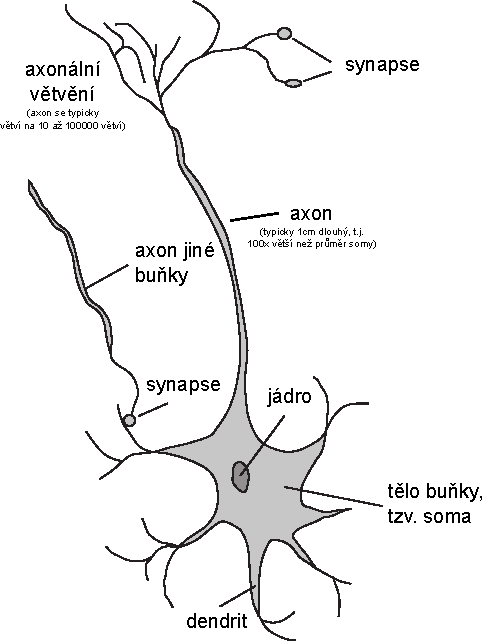
\includegraphics[width=11cm]{ML/neuron.pdf}
\end{center}
% 
% \begin{itemize}
%  \item dendritická struktura
%  \item tělo
%  \item axon
%  \item synapse
% \end{itemize}
% You have about neurons each with about weights. 
% – A huge number of weights can affect the computation in a very short 
% time. Much better bandwidth than a workstation.
% - 10^{11} neuronů, každý cca  10^4 vah
% - ačkoliv jsou synapse pomalé oproti RAM, vzhledem k jejich počtu mají mnohonásobně větší ``bandwith''
% - modularita
\end{frame}

\begin{frame}\frametitle{Matematický neuron --- $N: X_1\times\cdots\times X_n\to Y$}
\pause
 \begin{itemize}
  \item Lineární neurony
  \begin{displaymath}
   N(X) = b + \sum_{i=0}^n x_i w_i
  \end{displaymath}\pause
  \item Binární prahové neurony\pause
  \begin{itemize}
    \item McCulloch \& Pitts, 1943\pause
    \item spike $\approx$ pravdivostní hodnota výroku\pause
    \item neuron počítá se pravdivostní hodnotu jiného výroku ze vstupních výroků\pause
  \end{itemize}
  \item Lineární prahové neurony\pause
%     --- podobné ale nikoliv 0,1, spíše 0 nebo lineární
  \item Sigmoidy (logistická funkce, příp. tanh)\pause
  \begin{displaymath}
   N(X) = \frac{1}{1 + e^{-z}}\pause, z = b + \sum_{i=0}^n x_i w_i
  \end{displaymath}\pause
  \begin{itemize}
    \item mají hezké derivace\pause
    \item proto se s nimi dobře pracuje\pause
  \end{itemize}
  \item Stochastické neurony\pause
    \begin{itemize}
    \item výstup se interpretuje jako pravděpodobnost
    \end{itemize}
 \end{itemize}
\end{frame}

\begin{frame}\frametitle{Jednoduché rozpoznávání znaků}
\begin{itemize}
 \item dvouvrstvá síť\pause
 \item vstupní neurony = pixely\pause
 \item výstupní neurony = jednotlivé znaky\pause
 \item pixel může hlasovat pokud je zabarvený\pause
 \item pixel může hlasovat pro víc znaků\pause
 \item znak s největším počtem hlasů vyhrává\pause
\end{itemize}

\begin{center}
 Proces učení
\end{center}\pause
 V každém kroku:\pause
 \begin{itemize}
  \item zvyš váhy z aktivních pixelů do správné třídy\pause
  \item následně sniž váhy z aktivních pixelů do aktuálně uhádnuté třídy
 \end{itemize}
\end{frame}

\begin{frame}\frametitle{Rozpoznávání znaků --- učení v obrázcích}
\begin{center}
 \only<1>{\hskip4.2mm\includegraphics[width=10cm]{ML/2stage0.pdf}}
 \only<2>{\hskip2.8mm\includegraphics[width=10cm]{ML/2stage1.pdf}}
 \only<3>{\hskip1.4mm\includegraphics[width=10cm]{ML/2stage2.pdf}}
 \only<4>{\includegraphics[width=10cm]{ML/2stage3.pdf}}
 \only<5>{\includegraphics[width=10cm]{ML/2stage4.pdf}}
 \only<6>{\includegraphics[width=10cm]{ML/2stage5.pdf}}
\end{center}
\begin{center}
  {\tiny(zdroj: G. Hinton, Neural Networks for ML)}
\end{center}


\end{frame}


\begin{frame}\frametitle{Typy učících úloh}
\begin{itemize}
 \item řízené učení (supervised learning)\pause
    \begin{itemize}
      \item regrese\pause
      \item klasifikace\pause
    \end{itemize}
 \item reinforcement learning\pause
%  Learn to select an action to maximize payoff. 
 \item neřízené učení (unsupervised learning)
%  Discover a good internal representation of the input. 
%  PCA
% For about 40 years, unsupervised learning was largely ignored by the 
% machine learning community 
% – Some widely used definitions of machine learning actually excluded it. 
% – Many researchers thought that clustering was the only form of 
% unsupervised learning. 
% • It is hard to say what the aim of unsupervised learning is. 
% – One major aim is to create an internal representation of the input that 
% is useful for subsequent supervised or reinforcement learning. 
% – You can compute the distance to a surface by using the disparity 
% between two images. But you don’t want to learn to compute 
% disparities by stubbing your toe thousands of times. 
% Other goals for unsupervised learning
% • It provides a compact, low-dimensional representation of the input. 
% – High-dimensional inputs typically live on or near a lowdimensional manifold (or several such manifolds). 
% – Principal Component Analysis is a widely used linear method 
% for finding a low-dimensional representation. 
% • It provides an economical high-dimensional representation of the 
% input in terms of learned features. 
% – Binary features are economical. 
% – So are real-valued features that are nearly all zero. 
% • It finds sensible clusters in the input. 
% – This is an example of a very sparse code in which only one of 
% the features is non-zero. 
\end{itemize}
\end{frame}

\begin{frame}\frametitle{Typy neuronových sítí}
 \begin{itemize}
  \item feed forward\pause\ (hluboké --- >2 vnitřní vrstvy)\pause
  \item rekurentní neuronové sítě\pause
  \item symetrické (Hopfieldova síť)
 \end{itemize}
\end{frame}

\begin{frame}\frametitle{Síla rekurentních sítí}
\begin{center}
 I. Sutskever (2011) trénoval Neuronovou síť tak, aby uhodla následující znak v posloupnosti znaků.\pause\
 Trénovací data:\pause\ Wikipedie.\pause
\end{center}
\alert{Výsledek (generovaný po jednom znaku)}\pause

In 1974 Northern Denver had been
overshadowed by CNL, and several Irish
intelligence agencies in the Mediterranean
region. However, on the Victoria, Kings
Hebrew stated that Charles decided to
escape during an alliance. The mansion
house was completed in 1882, the second in
its bridge are omitted, while closing is the
proton reticulum composed below it aims,
such that it is the blurring of appearing on any
well-paid type of box printer.
\begin{center} 
 {\tiny(zdroj: G. Hinton, Neural Networks for ML)}
\end{center}
\end{frame}

\begin{frame}\frametitle{Perceptron}

\end{frame}

\begin{frame}\frametitle{Hopfieldova síť}
\end{frame}




\begin{frame}\frametitle{Zdroje}
\url{https://class.coursera.org/neuralnets-2012-001/}
\end{frame}

\end{document}